\documentclass[12pt]{article}%
\usepackage[paper=portrait,pagesize]{typearea}
\usepackage{amssymb}
\usepackage{amsfonts}
\usepackage{amsmath}
\usepackage{hyperref}
\usepackage{lscape}
\usepackage{comment}
\usepackage[flushleft]{threeparttable}
\usepackage{float}
\usepackage[nohead]{geometry}
\usepackage[singlespacing]{setspace}
\usepackage[paper=portrait,pagesize]{typearea}
\usepackage{amssymb}
\usepackage{amsfonts}
\usepackage{multicol}
\usepackage{amsmath}
\usepackage{hyperref}
\usepackage[nameinlink,noabbrev]{cleveref}
\usepackage{lscape}
\usepackage{float}
\usepackage[nohead]{geometry}
\usepackage[singlespacing]{setspace}
\usepackage[bottom]{footmisc}
\usepackage{indentfirst}
\usepackage{endnotes}
\usepackage{graphicx}%
\usepackage{afterpage}
\usepackage{subfig}
\usepackage{rotating}
\newcommand\tab[1][1cm]{\hspace*{#1}}
\DeclareMathOperator*{\Max}{Max}
\newcommand\numberthis{\addtocounter{equation}{1}\tag{\theequation}}
\def\dotfill#1{\cleaders\hbox to #1{.}\hfill}
\newcommand\dotline[2][.5em]{\leavevmode\hbox to #2{\dotfill{#1}\hfil}}
%\usepackage[backend=biber,style=alphabetic,sorting=ynt]{biblatex}
%\addbibresource{bibliocopulas.bib}
\usepackage[round,sort,comma,authoryear]{natbib}
\setcounter{MaxMatrixCols}{30}
\newtheorem{theorem}{Theorem}
\newtheorem{acknowledgement}{Acknowledgement}
\newtheorem{algorithm}[theorem]{Algorithm}
\newtheorem{axiom}[theorem]{Axiom}
\newtheorem{case}[theorem]{Case}
\newtheorem{claim}[theorem]{Claim}
\newtheorem{conclusion}[theorem]{Conclusion}
\newtheorem{condition}[theorem]{Condition}
\newtheorem{conjecture}[theorem]{Conjecture}
\newtheorem{corollary}[theorem]{Corollary}
\newtheorem{criterion}[theorem]{Criterion}
\newtheorem{definition}[theorem]{Definition}
\newtheorem{example}[theorem]{Example}
\newtheorem{exercise}[theorem]{Exercise}
\newtheorem{lemma}[theorem]{Lemma}
\newtheorem{notation}[theorem]{Notation}
\newtheorem{problem}[theorem]{Problem}
\newtheorem{proposition}{Proposition}
\newtheorem{remark}[theorem]{Remark}
\newtheorem{solution}[theorem]{Solution}
\newtheorem{summary}[theorem]{Summary}
\newenvironment{proof}[1][Proof]{\noindent\textbf{#1.} }{\ \rule{0.5em}{0.5em}}
\newcommand{\pd}[2]{\frac{\partial#1}{\partial#2}}
\makeatletter
\def\@biblabel#1{\hspace*{-\labelsep}}
\makeatother
\geometry{left=1in,right=1in,top=1.00in,bottom=1.0in}
%\renewcommand*\abstractname{Summary}

\begin{document}

\title{Fall 2019 - ECON 634 - Advance Macroeconomics - Problem Set 1}
\author{Elisa Taveras Pena\footnote{E-mail address: \href{mailto:etavera2@binghamton.edu}{etavera2@binghamton.edu}  }\\
Binghamton University}
\maketitle

\sloppy%avoids the breakage of words at the end of lines, by adjusting spaces between words inside the lines

\onehalfspacing

\begin{enumerate}
	\item Read the description of datasets in Olivetti et al (2012). Look in more detail at one of the datasets they describe. Explain which part of the data interests you, formulate a tentative research question, and find a recent (2015 or later) academic paper on a related topic that uses the data.
	    	\vspace{3mm}
	
	{\bf Answer}   	
	
	\vspace{3mm}
	
	I decided to explore more in depth the NLSY, which I went to the webpage and read further about. The reason for which it interested me is that my research focused on household economics, intrahousehold decisions, education and labor outcome and this dataset cover to some extend these. I feel familiar with the PSID so I wanted to explore a different dataset but focused on the individuals demographics ans life-cycle. NLSY has very detail information on the characteristic of the youth education attaintment, which definetly help to answer questions related to education mobility (i.e. how people move from public high school to private university) as well as how education relationship also relate to other demographics as marriage decisions and other marital demographics.
	
	\textbf{Research Question:}
	My research question is understanding how the education attainment of the women of the NLSY databases relate to the spouse's labor supply characteristics. Are more educated women marrying to certain occupation? are the characteristics of the education that they attained (i.e. Public or private education) move them to an specific partner's labor characteristics. Moreover, how this interaction has changed by cohort can be also studied since women's education attainment characteristics 
	
	The motivation for this is that the changes on the education attainment of couples, where now on average women are more educated than their husband (based on ACS statistics), which in part as been attributed to being because of gains that they will earn through the marriage market. 
	
	\textbf{Related paper:}
	
	Addo, Fenaba R.; Houle, Jason N.; Sassler, Sharon(2019). The Changing Nature of the Association between Student Loan Debt and Marital Behavior in Young Adulthood. 
	Journal of Family and Economic Issues, March 2019, v. 40, iss. 1, pp. 86-101.
	
	\item Read the reports by Díaz-Giménez, Glover, Rios-Rull (2011) and M. Kuhn and Rios-Rull (2015), and identify a graph or table that interests you
	(e.g., how is mobility related to education, age, marital status, etc; how is inequality at the top of the income distribution behaved; ...). Formulate a tentative research question and find a recent (2015 or later) academic  paper on a related topic.
	
		    	\vspace{3mm}
	
	{\bf Answer}   	
	
	\vspace{3mm}
	
	The part that interested the most to be was the one related to mobility, tables 27-29 of Díaz-Giménez, Glover, Rios-Rull (2011) report. Base on this I will keep following my discussion in term of marital relationship story. Two ideas comes to mind:
	
 \begin{itemize}
 	\item Understand how the couples relationship, measure as the women relative education within the marriage $\left( \frac{E_w}{E_h}\right) $ and how this relationship affect the mobility of the household. 
 	
 	\item Another possibility is analyze how remarried affects mobility. Since the PSID has information on those that remarriage and the time of marriage, it is possible to calculate the place in the income distribution that the marriage occupies for each number of the marriage and compare changed across marriages. In this way we can analyze how the household composition changes affects the mobility of the household. Are household in the second marriage having higher mobility than otherwise? 
 	
 \end{itemize}

	\textbf{Related papers:}


Ludwig, Johannes (2015). The Role of Education and Household Composition for Transitory and Permanent Income Inequality-Evidence from PSID Data. 
Journal of Macroeconomics, December 2015, v. 46, pp. 129-46

Gonalons-Pons, Pilar; Schwartz, Christine R. (2017). Trends in Economic Homogamy: Changes in Assortative Mating or the Division of Labor in Marriage?
Demography, June 2017, v. 54, iss. 3, pp. 985-1005
	
	
	\item EITHER replicate Tables 1 and 2 from DGR (2011) using the 2007 Survey of Consumer Finances, OR update their tables 1 and 2 using the more
	recent wave of the survey from 2013 (compare the results to Kuhn/Rios-	Rull). Follow the methodology as described in their text. Plot the Lorenz
	curves for earnings, income and wealth.
	
		    	\vspace{3mm}
	
	{\bf Answer}   	
	
	
	
	\begin {table}[H]
	\footnotesize
	\begin{center}
			\caption {Replication of Table 1 of DGR (2011)}
			\label{tab:Table1}
			{
				\begin{tabular}{l*{12}{l}}
					\hline
					Quantiles&  0&1&5&10&20&40&60&80&90&95&99&100\\
					\hline
					Earnings &-1,546.5 & 0&0 & 0&0&25.7&50.5&87.5& 126.1& 180.2&497&161,521.5\\
					Income   &-505.8  & 4.2 & 8.92& 12.34& 20.1&36.3& 58.8&98.72&141.98&207.21&680.68&187,200.5   \\
					Wealth   & -473.7 &-31.26 & -4.6&.03 & 7.33&64.9&197.9&496.9&910.3&1,900.17&8,374.5&   1,411,730 \\
					\hline
				\end{tabular}
			}	

	\end{center} 
	\end {table}

\normalfont

	\begin {table}[H]
\footnotesize
\begin{center}
	\caption {Replication of Table 2 of DGR (2011)}
	\label{tab:Table2}
	{
		\begin{tabular}{l*{3}{c}}
			\hline
			&  Earnings&Income&Wealth\\
			\hline
			Coefficient of Variation &  3.61 &   4.32 &  6.01\\
			Variance of the logs  &1.288 & .992 4.532	 \\
			Gini index & 0.63580.57498&0.8162\\
			Top 1 \% /  Top 40\%&&&\\
			\multicolumn{4}{l}{\dotline[2pt]{10cm}} \\
			Location of the mean (\%) &69&74&81\\
			Mean/Median & 1.724 &	1.767 & 4.601\\
			\hline
		\end{tabular}
	}	
	
\end{center} 
\end {table}
	
	\vspace{3mm}
	
	
	Finally, The Lorenz Curves will looks as follows:
	   \begin{figure}[H]
		\begin{center}
			\begin{multicols}{3}
				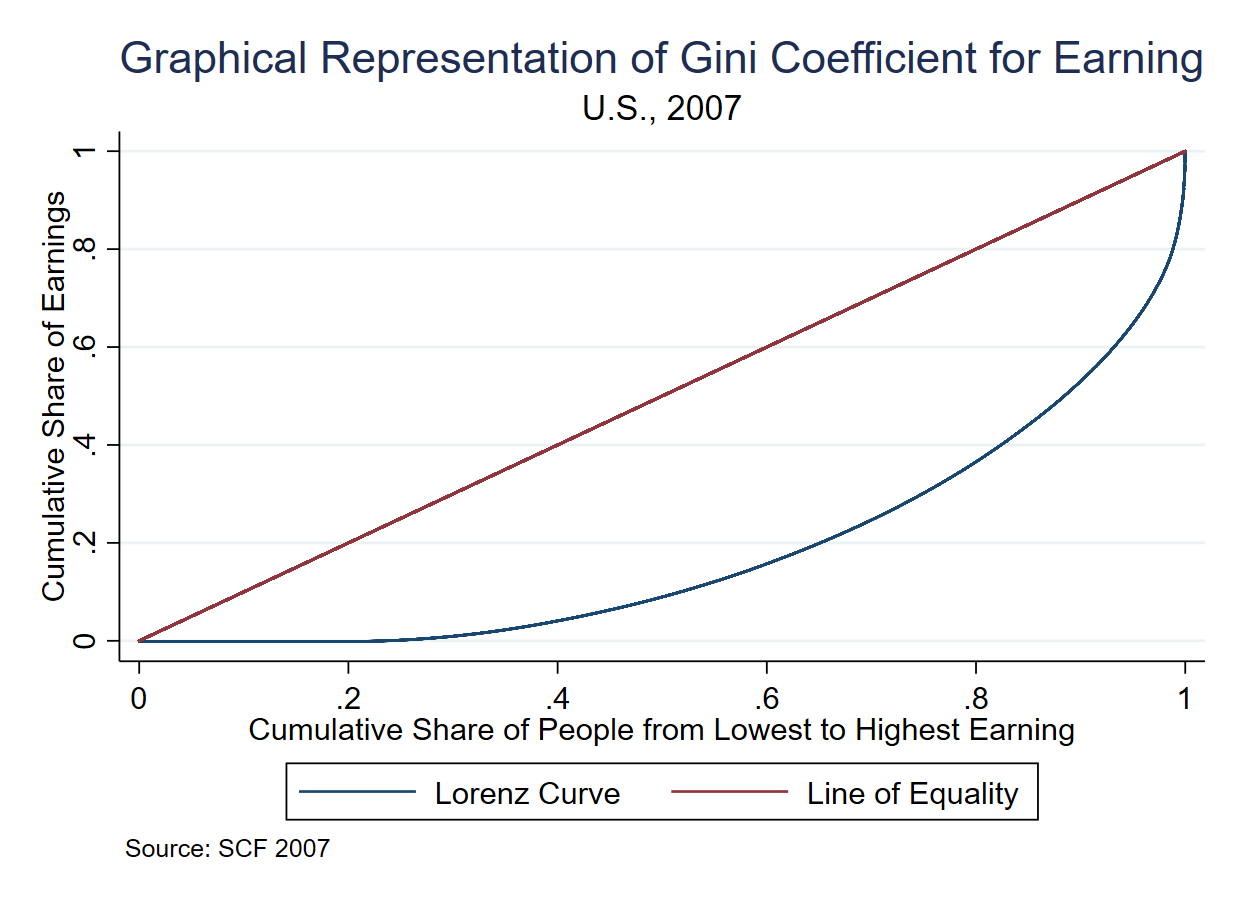
\includegraphics[width=0.9\linewidth]{build_data/output/Lorenz_earning}
				\columnbreak
				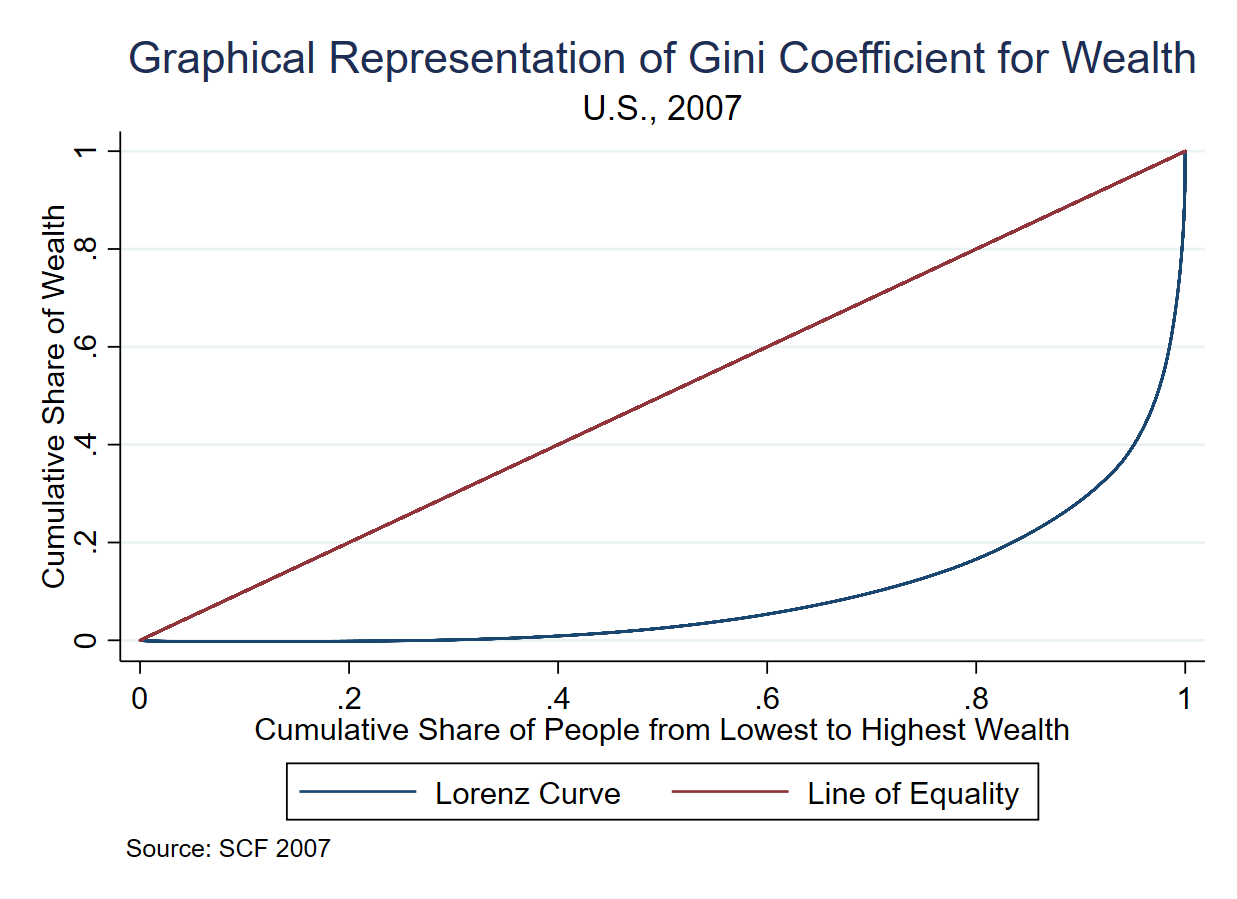
\includegraphics[width=0.9\linewidth]{build_data/output/Lorenz_wealth}
				\columnbreak
				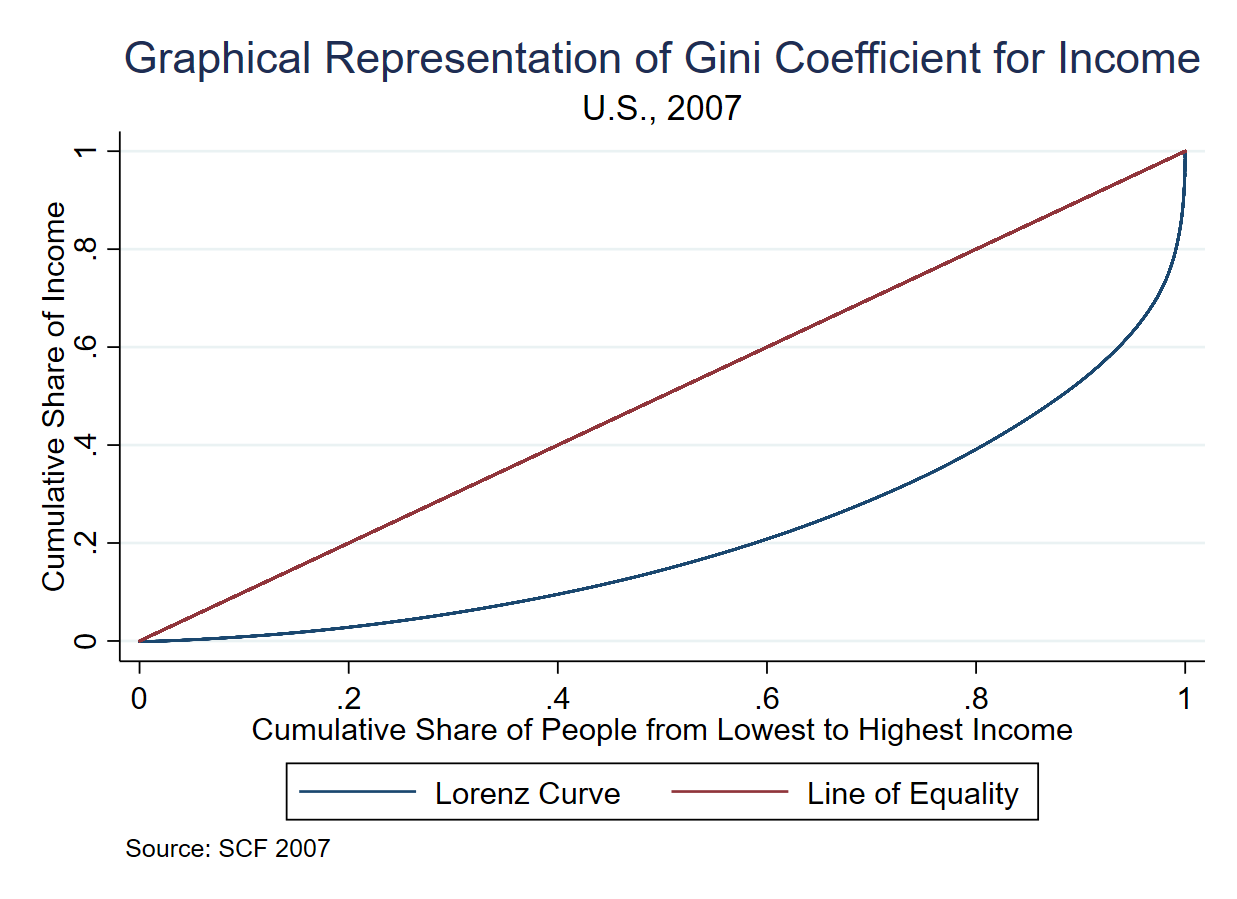
\includegraphics[width=0.9\linewidth]{build_data/output/Lorenz_income}
				\columnbreak
			\end{multicols}
		\end{center}	
		\caption{\small \sl Lorenz curves} 
		\label{fig:Fig1}
	\end{figure}
	
	
	
\end{enumerate}

\strut

\onehalfspacing

\end{document}
